\ifx\wholebook\relax \else
% ------------------------

\documentclass{ctexart}
\usepackage[cn]{../../../prelude}

\setcounter{page}{1}

\begin{document}

%--------------------------

% ================================================================
%                 COVER PAGE
% ================================================================

\title{红黑树的命令式删除算法}

\author{刘新宇
\thanks{{\bfseries 刘新宇} \newline
  Email: liuxinyu95@gmail.com \newline}
  }

\maketitle
\fi

\markboth{红黑树}{初等算法}

\ifx\wholebook\relax
\chapter{红黑树的命令式删除算法}
\numberwithin{Exercise}{chapter}
\fi

% ================================================================
%                 Introduction
% ================================================================
\index{红黑树!命令式删除}

本附录包含红黑树的命令式删除算法。我们需要在普通二叉搜索树删除算法的基础上,通过旋转和重新染色恢复红黑树的性质,以保持树的平衡。我们在红黑树一章中指出,当删除黑色节点时,会破坏红黑树的第五条性质。使得某一路径上的黑色节点数目减少。为此,我们引入“双重黑色”节点,来保持所删除路径上的黑色节点数目不变。

\section{双重黑色}
\index{红黑树!双重黑色}

为了支持“双重黑色”的节点,我们需要增加颜色的定义。如下面的C++例子代码所示。

\lstset{language=C++}
\begin{lstlisting}
enum class Color { RED, BLACK, DOUBLY_BLACK };
\end{lstlisting}

在删除一个节点时,我们复用二叉搜索树的删除算法,并记录被删除节点的父节点。如果被删除节点的颜色是黑色我们需要通过处理保持黑色的属性,然后再进行进一步修复。

\begin{algorithmic}[1]
\Function{Delete}{$T, x$}
  \State $p \gets$ \Call{Parent}{$x$}
  \State $q \gets$ NIL
  \If{\Call{Left}{$x$} = NIL}
    \State $q \gets$ \Call{Right}{$x$}
    \State replace $x$ with \Call{Right}{$x$}
  \ElsIf{\Call{Right}{$x$} = NIL}
    \State $q \gets$ \Call{Left}{$x$}
    \State replace $x$ with \Call{Left}{$x$}
  \Else
    \State $y \gets$ \textproc{Min}(\Call{Right}{$x$})
    \State $p \gets$ \Call{Parent}{$y$}
    \State $q \gets$ \Call{Right}{$y$}
    \State \Call{Key}{$x$} $\gets$ \Call{Key}{$y$}
    \State copy satellite data from $y$ to $x$
    \State replace $y$ with \Call{Right}{$y$}
    \State $x \gets y$
  \EndIf
  \If{\Call{Color}{$x$} = BLACK}
    \State $T \gets$ \textproc{Delete-Fix}($T$, \Call{Make-Black}{$p$, $q$}, $q$ = NIL?)
  \EndIf
  \State release $x$
  \State \Return $T$
\EndFunction
\end{algorithmic}

删除算法接受树的根节点$T$和待删除节点$x$。如果待删除节点存在一个为空的分支,我们可以将$x$“切下”,并用另一个分支$q$来替代$x$。否则,我们在$x$的右子树中找到最小的节点$y$,用$y$替换$x$。然后递归地将$y$“切下”。如果被删除的节点$x$的颜色为黑色,我们调用\textproc{Make-Black}($p$, $q$),来保持黑色属性,以便进行下一步的修复。

\begin{algorithmic}[1]
\Function{Make-Black}{$p$, $q$}
  \If{$p$ = NIL $\land$ $q$ = NIL}
    \State \Return NIL \Comment{删除只有一个叶子节点的树后,变为空}
  \ElsIf{$q$ = NIL}
    \State $n \gets$ Doubly Black NIL
    \State \Call{Parent}{$n$} $\gets p$
    \State \Return $n$
  \Else
    \State \Return \Call{Blacken}{$q$}
  \EndIf
\EndFunction
\end{algorithmic}

如果传入\textproc{Make-Black}的参数$p$和$q$都为空,说明我们在删除只有一个叶子节点的树,删除后树变为空。否则如果父节点$p$不为空,而节点$q$为空。说明我们删除了一个黑色的叶子节点。这相当于,此时一个NIL节点替换了被删除的黑色节点。根据红黑树的性质3,NIL节点实际上都是黑色的。我们可以把这一NIL节点变成“双重黑色”NIL节点来保持其所在路径上的黑色节点数目不变。最后,如果$p$、$q$都不为空,我们调用\textproc{Blacken}检查$q$的颜色,如果是红色的,将它重新染成黑色,如果$q$已经是黑色的,我们将它染成双重黑色。

\subsection{修复}

为了最终恢复红黑树的性质,我们需要通过树的旋转操作和重新染色,最终去掉“双重黑色”。这里有三种情况需要处理(\cite{CLRS}第292页)。每一种情况中,双重黑色的节点即可以是普通节点,也可以是双重黑色的空节点。我们首先看第一种情况。

\subsection{双重黑色节点的兄弟为黑色,并且该兄弟节点有一个红色子节点}
对于这种情况,我们可以通过旋转操作来修复。总共有四种不同的细分情况,它们全部可以变换到一种统一的形式。如图\ref{fig:del-case1}所示。

\begin{figure}[htbp]
   \centering
   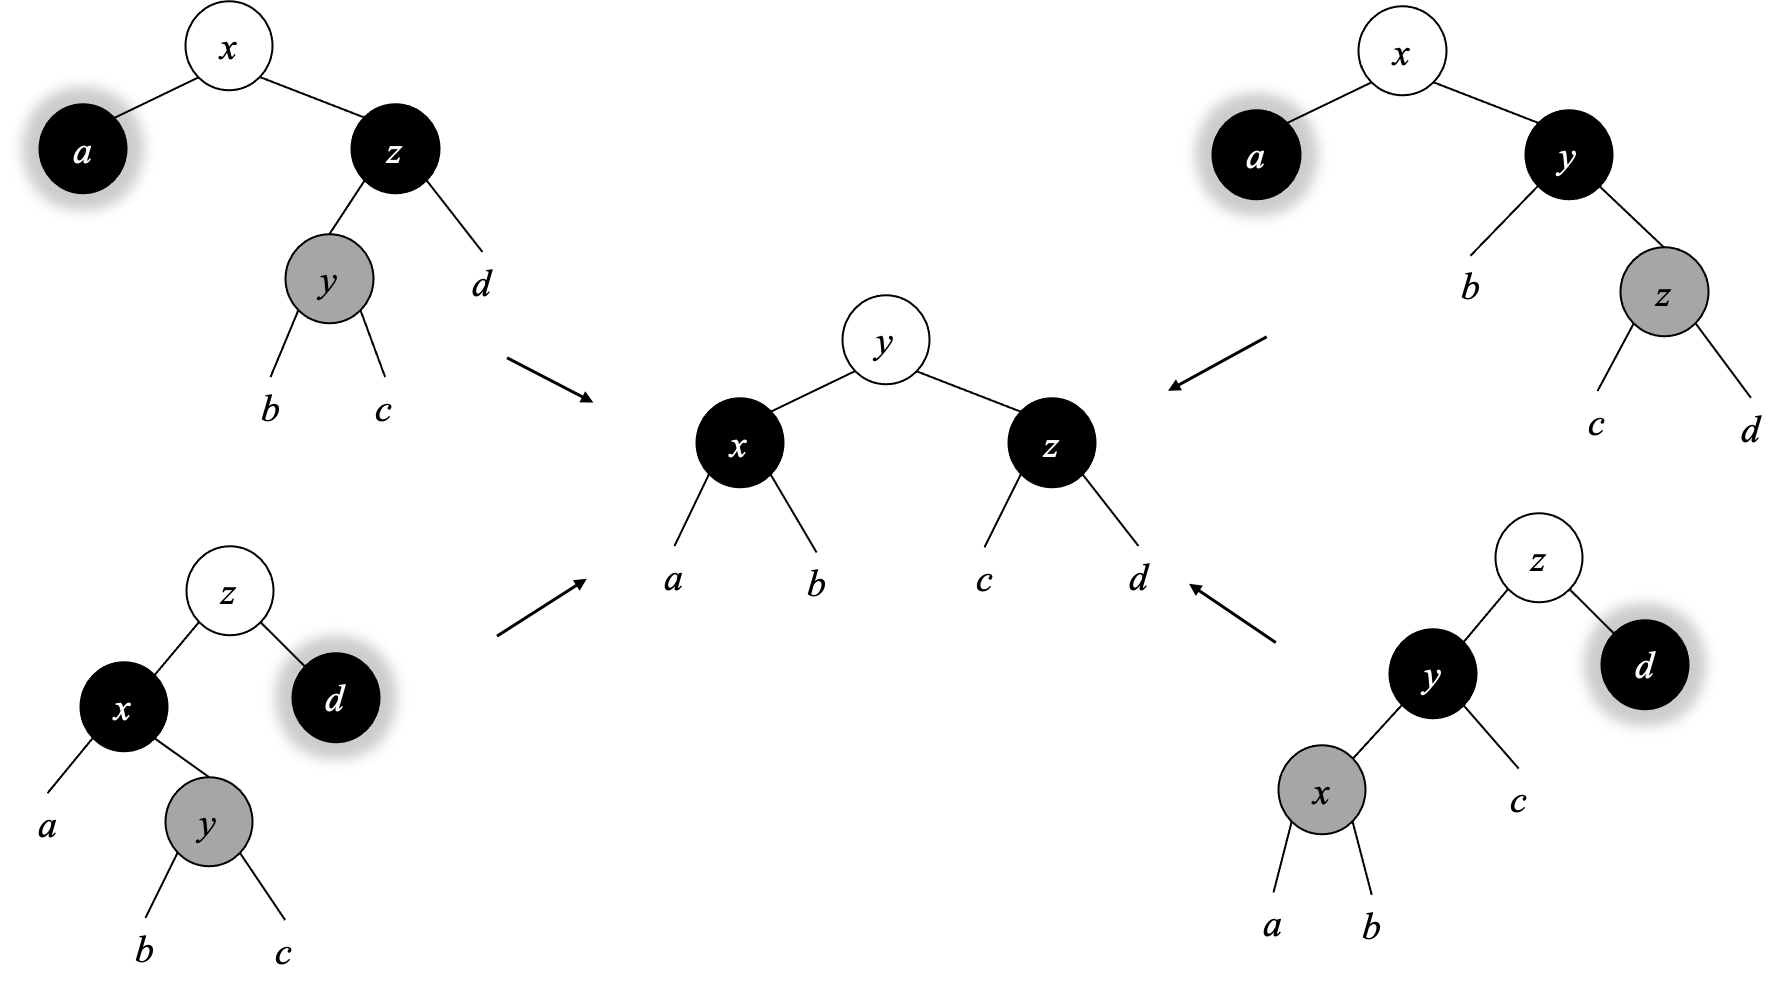
\includegraphics[scale=0.4]{../../../datastruct/tree/red-black-tree/img/del-case1.eps}
   \caption{双重黑色节点的兄弟为黑色,并且该兄弟节点有一个红色子节点。这种情况可以通过一次旋转操作来修复。}
   \label{fig:del-case1}
\end{figure}

下面的算法描述了针对这一情况的处理。

\begin{algorithmic}[1]
\Function{Delete-Fix}{$T$, $x$, $f$}
  \State $n \gets$ NIL
  \If{$f$ = True}  \Comment{$x$是一个双重黑色NIL节点}
    \State $n \gets x$
  \EndIf
  \If{$x$ = NIL} \Comment{将只有一个叶子节点的树删空}
    \State \Return NIL
  \EndIf
  \While{$x \neq T \land$ \Call{Color}{$x$} $= \mathcal{B}^2$}
    \Comment{$x$不是根且$x$是双重黑色}
    \If{\Call{Sibling}{$x$} $\neq$ NIL} \Comment{双重黑色节点的兄弟节点不为空}
        \State $s \gets$ \Call{Sibling}{$x$}
        \State ...
        \If{$s$ is black $\land$ \Call{Left}{$s$} is red}
          \Comment{兄弟为黑,一个侄子为红}
          \If{$x = $ \textproc{Left}(\Call{Parent}{$x$})}
            \Comment{$x$在左侧}
            \State set $x$, \Call{Parent}{$x$}, and \Call{Left}{$s$} all black
            \State $T \gets$ \Call{Rotate-Right}{$T$, $s$}
            \State $T \gets$ \textproc{Rotate-Left}($T$, \Call{Parent}{$x$})
          \Else \Comment{$x$在右侧}
            \State set $x$, \Call{Parent}{$x$}, $s$, and \Call{Left}{$s$} all black
            \State $T \gets$ \textproc{Rotate-Right}($T$, \Call{Parent}{$x$})
          \EndIf
        \ElsIf{$s$ is black $\land$ \Call{Right}{$s$} is red}
          \Comment{兄弟为黑,一个侄子为红}
          \If{$x = $ \textproc{Left}(\Call{Parent}{$x$})} \Comment{$x$在左侧}
            \State set $x$, \Call{Parent}{$x$}, $s$, and \Call{Right}{$s$} all black
            \State $T \gets$ \textproc{Rotate-Left}($T$, \Call{Parent}{$x$})
          \Else \Comment{$x$在右侧}
            \State set $x$, \Call{Parent}{$x$}, and \Call{Right}{$s$} all black
            \State $T \gets$ \Call{Rotate-Left}{$T$, $s$}
            \State $T \gets$ \textproc{Rotate-Right}($T$, \Call{Parent}{$x$})
          \EndIf
        \State ...
        \EndIf
    \EndIf
  \EndWhile
\EndFunction
\end{algorithmic}

\subsection{双重黑色节点的兄弟节点为红色}
这种情况下,我们可以通过旋转,将双重黑色恢复为普通的黑色节点。如图\ref{fig:del-case2}所示,将左侧的树旋转到右侧的结构后,可将双重黑色的节点$a$或$c$恢复为黑色。

\begin{figure}[htbp]
  \centering
  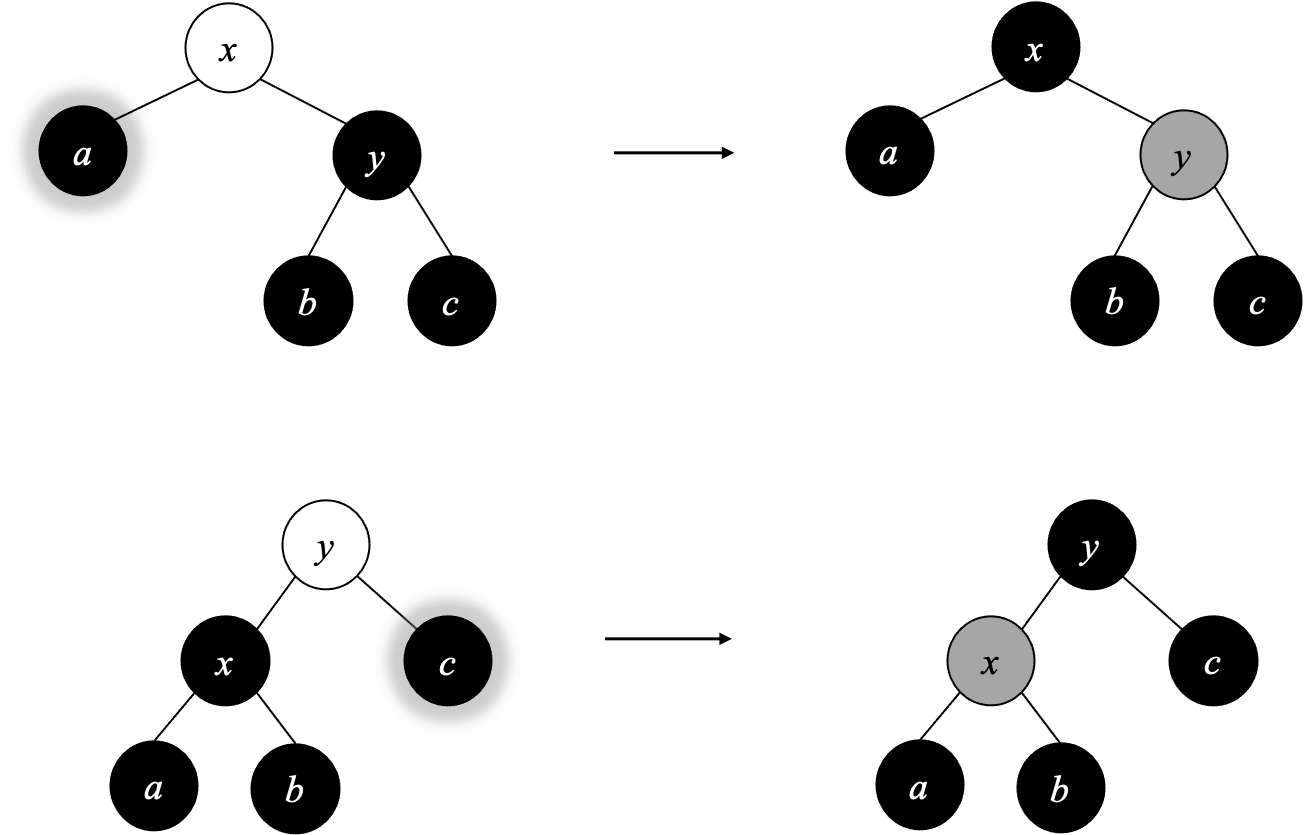
\includegraphics[scale=0.4]{../../../datastruct/tree/red-black-tree/img/del-case3.eps}
  \caption{双重黑色节点的兄弟节点为红色} \label{fig:del-case2}
\end{figure}

我们在此前给出算法上增加这一处理。

\begin{algorithmic}[1]
\Function{Delete-Fix}{$T$, $x$, $f$}
  \State $n \gets$ NIL
  \If{$f$ = True}  \Comment{$x$是一个双重黑色NIL节点}
    \State $n \gets x$
  \EndIf
  \If{$x$ = NIL} \Comment{将只有一个叶子节点的树删空}
    \State \Return NIL
  \EndIf
  \While{$x \neq T \land$ \Call{Color}{$x$} $= \mathcal{B}^2$}
    \Comment{$x$不是根且$x$是双重黑色}
    \If{\Call{Sibling}{$x$} $\neq$ NIL} \Comment{双重黑色节点的兄弟节点不为空}
        \State $s \gets$ \Call{Sibling}{$x$}
        \If{$s$ is red} \Comment{兄弟为红色}
          \State set \Call{Parent}{$x$} red
          \State set $s$ black
          \If{$x = $ \textproc{Left}(\Call{Parent}{$x$})} \Comment{$x$在左侧}
            \State $T \gets$ \textproc{Rotate-Left}{$T$, \Call{Parent}{$x$}}
          \Else \Comment{$x$在右侧}
            \State $T \gets$ \textproc{Rotate-Right}{$T$, \Call{Parent}{$x$}}
          \EndIf
        \ElsIf{$s$ is black $\land$ \Call{Left}{$s$} is red}
          \Comment{兄弟为黑,一个侄子为红}
          \State ...
        \EndIf
    \EndIf
  \EndWhile
\EndFunction
\end{algorithmic}

\subsection{双重黑色节点的兄弟节点为黑色,该兄弟节点的两个子节点也全是黑色。}
这种情况下,我们可以将这个兄弟节点染成红色,将双重黑色变回黑色,然后将双重黑色属性向上传递一层到父节点。如图\ref{fig:del-case3}所示,有两种对称的情况。

\begin{figure}[htbp]
  \centering
  \setlength{\unitlength}{1cm}
  \begin{picture}(10, 4)
  \put(5, 2){$\Rightarrow$}
  \subcaptionbox{$x$的颜色为红或者黑。}{\includegraphics[scale=0.4]{../../../datastruct/tree/red-black-tree/img/case2-a.ps}}
  \subcaptionbox{若$x$此前的颜色为红,将其变为黑色,否则变为双重黑色。}{\includegraphics[scale=0.4]{../../../datastruct/tree/red-black-tree/img/case2-a1.ps}}
  \end{picture}
  \\
  \begin{picture}(10, 5)
  \put(5, 2){$\Rightarrow$}
  \subcaptionbox{$y$的颜色为红或者黑。}{\includegraphics[scale=0.4]{../../../datastruct/tree/red-black-tree/img/case2-b.ps}}
  \subcaptionbox{若$y$此前的颜色为红,将其变为黑色,否则变为双重黑色。}{\includegraphics[scale=0.4]{../../../datastruct/tree/red-black-tree/img/case2-b1.ps}}
  \end{picture}
  \\
  \begin{picture}(1, 0.5)\end{picture} %pad
  \caption{将双重黑色向上传递} \label{fig:del-case3}
\end{figure}

上述三种情况中,双重黑色节点的兄弟节点都不为空。如果其兄弟节点为空,我们可以直接将双重黑色恢复为普通黑色,然后将黑色向上传递。如果双重黑色最终向上传递到根节点,我们可以将根节点变为普通黑色节点,从而结束修复过程。另外,如果双重黑色在修复过程中被重新染色为普通节点,我们也可以终止。最后,我们需要一个额外处理,即如果最终的双重黑色节点是一个双重黑色空节点,我们需要将其恢复为普通空节点。最终的算法如下所示。

\begin{algorithmic}[1]
\Function{Delete-Fix}{$T$, $x$, $f$}
  \State $n \gets$ NIL
  \If{$f$ = True}  \Comment{$x$是一个双重黑色NIL节点}
    \State $n \gets x$
  \EndIf
  \If{$x$ = NIL} \Comment{将只有一个叶子节点的树删空}
    \State \Return NIL
  \EndIf
  \While{$x \neq T \land$ \Call{Color}{$x$} $= \mathcal{B}^2$}
    \Comment{$x$不是根且$x$是双重黑色}
    \If{\Call{Sibling}{$x$} $\neq$ NIL} \Comment{双重黑色节点的兄弟节点不为空}
        \State $s \gets$ \Call{Sibling}{$x$}
        \If{$s$ is red} \Comment{兄弟为红色}
          \State set \Call{Parent}{$x$} red
          \State set $s$ black
          \If{$x = $ \textproc{Left}(\Call{Parent}{$x$})} \Comment{$x$在左侧}
            \State $T \gets$ \textproc{Rotate-Left}{$T$, \Call{Parent}{$x$}}
          \Else \Comment{$x$在右侧}
            \State $T \gets$ \textproc{Rotate-Right}{$T$, \Call{Parent}{$x$}}
          \EndIf
        \ElsIf{$s$ is black $\land$ \Call{Left}{$s$} is red}
          \Comment{兄弟为黑,一个侄子为红}
          \If{$x = $ \textproc{Left}(\Call{Parent}{$x$})}
            \Comment{$x$在左侧}
            \State set $x$, \Call{Parent}{$x$}, and \Call{Left}{$s$} all black
            \State $T \gets$ \Call{Rotate-Right}{$T$, $s$}
            \State $T \gets$ \textproc{Rotate-Left}($T$, \Call{Parent}{$x$})
          \Else \Comment{$x$在右侧}
            \State set $x$, \Call{Parent}{$x$}, $s$, and \Call{Left}{$s$} all black
            \State $T \gets$ \textproc{Rotate-Right}($T$, \Call{Parent}{$x$})
          \EndIf
        \ElsIf{$s$ is black $\land$ \Call{Right}{$s$} is red}
          \Comment{兄弟为黑,一个侄子为红}
          \If{$x = $ \textproc{Left}(\Call{Parent}{$x$})}
            \Comment{$x$在左侧}
            \State set $x$, \Call{Parent}{$x$}, $s$, and \Call{Right}{$s$} all black
            \State $T \gets$ \textproc{Rotate-Left}($T$, \Call{Parent}{$x$})
          \Else \Comment{$x$在右侧}
            \State set $x$, \Call{Parent}{$x$}, and \Call{Right}{$s$} all black
            \State $T \gets$ \Call{Rotate-Left}{$T$, $s$}
            \State $T \gets$ \textproc{Rotate-Right}($T$, \Call{Parent}{$x$})
          \EndIf
        \ElsIf{$s$, \Call{Left}{$s$}, and \Call{Right}{$s$} are all black}
          \Comment{兄弟和侄子都为黑色}
          \State set $x$ black
          \State set $s$ red
          \State \textproc{Blacken}(\Call{Parent}{$x$})
          \State $x \gets$ \Call{Parent}{$x$}
        \EndIf
    \Else \Comment{无兄弟节点,将黑色向上传递}
      \State set $x$ black
      \State \textproc{Blacken}(\Call{Parent}{$x$})
      \State $x \gets$ \Call{Parent}{$x$}
    \EndIf
  \EndWhile
  \State set $T$ black
  \If{$n \neq$ NIL} \Comment{替换双重黑色的NIL节点为普通NIL}
    \State replace $n$ with NIL
  \EndIf
  \State \Return $T$
\EndFunction
\end{algorithmic}

删除修复时,传入了三个参数,一个是树的根节点$T$;一个是待修复的节点$x$,它可能是双重黑色的节点;还有一个标记$f$,如果带修复的节点$x$是双重黑色的空节点NIL,则$f$为真。此时我们用$n$来记录这一双重黑色的空节点NIL,并且在最终修复完毕后,用普通NIL替换掉$n$。

下面的C++例子程序实现了红黑树的删除算法。

\lstset{language=C++}
\begin{lstlisting}
Node* del(Node* t, Node* x) {
    if (!x) return t;
    Node* parent = x->parent;
    Node* db = nullptr;        //doubly black
    Node* y;

    if (x->left == nullptr) {
        db = x->right;
        x->replaceWith(db);
    } else if (x->right == nullptr) {
        db = x->left;
        x->replaceWith(db);
    } else {
        y = min(x->right);
        parent = y->parent;
        db = y->right;
        x->key = y->key;
        y->replaceWith(db);
        x = y;
    }
    if (x->color == Color::BLACK)
        t = deleteFix(t, makeBlack(parent, db), db == nullptr);
    remove(x);
    return t;
}
\end{lstlisting}

其中\texttt{makeBlack}函数检查删除后节点是否变为双重黑色,并处理双重黑色空节点NIL的特殊情况。

\begin{lstlisting}
Node* makeBlack(Node* parent, Node* x) {
    if (!parent && ! x)
        return nullptr;
    if (!x)
        return Node::replace(parent, x, new Node(0, Color::DOUBLY_BLACK));
    return blacken(x);
}
\end{lstlisting}

其中函数\texttt{replace(parent, x, y)}将\texttt{parent}的子节点\texttt{x},用\texttt{y}替换。

\begin{lstlisting}
static Node* replace(Node* parent, Node* x, Node* y) {
    if (parent == nullptr) {
        if (y) y->parent = nullptr;
    } else if (parent->left == x) {
        parent->setLeft(y);
    } else {
        parent->setRight(y);
    }
    if (x) x->parent = nullptr;
    return y;
}
\end{lstlisting}

函数\texttt{blacken(node)}将红色节点染为黑色,将黑色节点染为双重黑色。

\begin{lstlisting}
Node* blacken(Node* x) {
    x->color = isRed(x) ? Color::BLACK : Color::DOUBLY_BLACK;
    return x;
}
\end{lstlisting}

最终的修复过程的实现如下。

\begin{lstlisting}
Node* deleteFix(Node* t, Node* db, bool isDBEmpty) {
    Node* dbEmpty = isDBEmpty ? db : nullptr;
    if (!db) return nullptr;    // remove the root from a leaf tree;
    while (db != t && db->color == Color::DOUBLY_BLACK) {
        if (db->sibling() != nullptr) {
            if (isRed(db->sibling())) {
                // the sibling is red, (transform to make the sibling black)
                setColors(db->parent, Color::RED,
                          db->sibling(), Color::BLACK);
                if (db == db->parent->left)
                    t = leftRotate(t, db->parent);
                else
                    t = rightRotate(t, db->parent);
            } else if (isBlack(db->sibling()) && isRed(db->sibling()->left)) {
                // the sibling is black, and one nephew is red
                if (db == db->parent->left) {
                    setColors(db, Color::BLACK,
                              db->parent, Color::BLACK,
                              db->sibling()->left, db->parent->color);
                    t = rightRotate(t, db->sibling());
                    t = leftRotate(t, db->parent);
                } else {
                    setColors(db, Color::BLACK,
                              db->parent, Color::BLACK,
                              db->sibling(), db->parent->color,
                              db->sibling()->left, Color::BLACK);
                    t = rightRotate(t, db->parent);
                }
            } else if (isBlack(db->sibling()) && isRed(db->sibling()->right)) {
                if (db == db->parent->left) {
                    setColors(db, Color::BLACK,
                              db->parent, Color::BLACK,
                              db->sibling(), db->parent->color,
                              db->sibling()->right, Color::BLACK);
                    t = leftRotate(t, db->parent);
                } else {
                    setColors(db, Color::BLACK,
                              db->parent, Color::BLACK,
                              db->sibling()->right, db->parent->color);
                    t = leftRotate(t, db->sibling());
                    t = rightRotate(t, db->parent);
                }
            } else if (isBlack(db->sibling()) &&
                       isBlack(db->sibling()->left) &&
                       isBlack(db->sibling()->right)) {
                // the sibling and both nephews are black.
                // move the blackness up
                setColors(db, Color::BLACK,
                          db->sibling(), Color::RED);
                blacken(db->parent);
                db = db->parent;
            }
        } else { // no sibling, move the blackness up
            db->color = Color::BLACK;
            blacken(db->parent);
            db = db->parent;
        }
    }
    t->color = Color::BLACK;
    if (dbEmpty) { // change the doubly black nil to nil
        dbEmpty->replaceWith(nullptr);
        delete dbEmpty;
    }
    return t;
}
\end{lstlisting}

其中\texttt{isBlack(node)}判断一个节点是否为黑色,根据红黑树的性质,所有的NIL节点的颜色为黑色。

\begin{lstlisting}
bool isBlack(Node* x) {
    return x == nullptr || x->color == Color::BLACK;
}

bool isRed(Node* x) {
    return x != nullptr && x->color == Color::RED;
}
\end{lstlisting}

函数\texttt{setColors}为一组辅助函数,用于对节点染色。

\begin{lstlisting}
void setColors(Node* x, Color a, Node* y, Color b) { x->color = a; y->color = b; }

void setColors(Node* x, Color a, Node* y, Color b, Node* z, Color c) {
    setColors(x, a, y, b);
    z->color = c;
}

void setColors(Node* x, Color a, Node* y, Color b,
               Node* z, Color c, Node* q, Color d) {
    setColors(x, a, y, b);
    setColors(z, c, q, d);
}
\end{lstlisting}

算法在结束前修复双重黑色空节点NIL时,调用节点的\texttt{replaceWith}方法,它通过调用前面定义的\texttt{replace}函数实现。

\begin{lstlisting}
void replaceWith(Node* y) {
    replace(parent, this, y);
}
\end{lstlisting}

考虑红黑树的平衡性,删除算法或者到达根节点终止,或者双重黑色消失终止。对于含有$n$个节点的红黑树,删除算法的复杂度为$O(\lg n)$。

\begin{Exercise}

\begin{itemize}
\item 选择一种命令式编程语言,实现完整的红黑树删除算法。
\item 选择一种命令式编程语言,编写程序判断一个给定的红黑树是否满足红黑树的5条性质,并用这一程序测试红黑树的删除算法。
\end{itemize}

\end{Exercise}

\ifx\wholebook\relax \else
\begin{thebibliography}{99}

\bibitem{CLRS}
Thomas H. Cormen, Charles E. Leiserson, Ronald L. Rivest and Clifford Stein.
``Introduction to Algorithms, Second Edition''. ISBN:0262032937. The MIT Press. 2001 (《算法导论》中文版)

\end{thebibliography}

\end{document}
\fi
